\documentclass{ximera}
\newcommand{\RR}{\mathbb R}
\renewcommand{\d}{\,d}
\newcommand{\dd}[2][]{\frac{d #1}{d #2}}
\renewcommand{\l}{\ell}
\newcommand{\ddx}{\frac{d}{dx}}
\newcommand{\dfn}{\textbf}
\newcommand{\eval}[1]{\bigg[ #1 \bigg]}


\outcome{Find the bounded area between two curves.}
\outcome{Integrate with respect to $y$.}
\outcome{Decided whether to integrate with respect to $x$ or $y$.}


\title[Dig-In:]{Area between curves}

\begin{document}
\begin{abstract}
  We compute the area of a region between two curves using the
  definite integral.
\end{abstract}
\maketitle


We have seen how integration can be used to find signed area between a
curve and the $x$-axis. With very little change we can find areas
bounded between curves.  Generally we should interpret ``area'' in the
usual sense, as a necessarily positive quantity. Suppose $f(x)>g(x)$
for all $x$ on the interval $[a,b]$ and we wish to know the geometric
area bounded between $f$ and $g$ on this interval:
\begin{image}
\begin{tikzpicture}
	\begin{axis}[
            domain=.5:2.5, ymax=10,xmax=2.5,ymin=0, xmin=.5,
            axis lines =left, xlabel=$x$, ylabel=$y$,
            xtick={1,2},
            ytick style={draw=none},
            width=4in,
            height=2in,
            yticklabels={},
            xticklabels={$a$, $b$},
            every axis y label/.style={at=(current axis.above origin),anchor=south},
            every axis x label/.style={at=(current axis.right of origin),anchor=west},
            axis on top,
          ]
          \addplot [draw=none,fill=fillp,domain=1:2] {-x^2+4*x+3} \closedcycle;
          \addplot [draw=none,fill=background,domain=1:2] {-x^3 + 7*x^2-10*x+5} \closedcycle;
          \addplot [draw=penColor,very thick] {-x^2+4*x+3};
          \addplot [draw=penColor2,very thick] {-x^3 + 7*x^2-10*x+5};
          \node at (axis cs:1,6.7) [penColor] {$f$};
          \node at (axis cs:2,4) [penColor2] {$g$};
        \end{axis}
\end{tikzpicture}
\end{image}
From the graph above we see that the area we want is the area under
$f$ minus the area under $g$, which is to say
\begin{align*}
\mathrm{Area} &= \int_a^b f(x)\d x-\int_a^b g(x)\d x \\
&= \int_a^b f(x)-g(x) \d x.
\end{align*}
It will also be useful to adopt the following intuitive way of
thinking about this problem: In a somewhat nonrigorous way, we can
think of an integral as ``summing up" an infinite number of
infinitesimal quantities. In this case we are summing rectangles of
width $\d x$ and height $f(x)-g(x)$:
\begin{image}
\begin{tikzpicture}
	\begin{axis}[
            domain=.5:2.5, ymax=10,xmax=2.5,ymin=0, xmin=.5,
            axis lines =left, xlabel=$x$, ylabel=$y$,
            xtick={1,2}, yticklabels={},
            ytick style={draw=none},
            xticklabels={$a$, $b$},
            width=4in,
            height=2in,
            every axis y label/.style={at=(current axis.above origin),anchor=south},
            every axis x label/.style={at=(current axis.right of origin),anchor=west},
            axis on top,
          ]
          %\addplot [draw=none,fill=fillp,domain=1:2] {-x^2+4*x+3} \closedcycle;
          %\addplot [draw=none,fill=background,domain=1:2] {-x^3 + 7*x^2-10*x+5} \closedcycle;
          \addplot [draw=penColor,very thick] {-x^2+4*x+3};
          \addplot [draw=penColor2,very thick] {-x^3 + 7*x^2-10*x+5};
          \node at (axis cs:1,6.7) [penColor] {$f$};
          \node at (axis cs:2,4) [penColor2] {$g$};
          \addplot [draw=penColor, fill = fillp] plot coordinates {(1.5,2.375) (1.6,2.375) (1.6, 6.84) (1.5,6.84) (1.5, 2.375)};
          
          \draw[decoration={brace,mirror,raise=.2cm},decorate,thin] (axis cs:1.5,2.7)--(axis cs:1.6,2.7);
          \node at (axis cs:1.55,1.25) {$\d x$};

          \draw[decoration={brace,raise=.2cm},decorate,thin] (axis cs:1.51,2.375)--(axis cs:1.51,6.84);
          \node[anchor=east] at (axis cs:1.45,4.6) {$f(x)-g(x)$};
        \end{axis}
\end{tikzpicture}
\end{image}
In this case, the integral
\begin{image}
  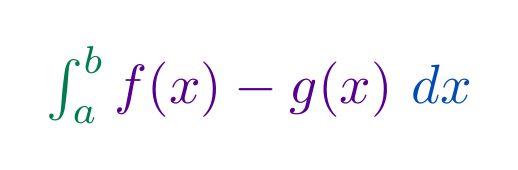
\begin{tikzpicture}[scale=2,every node/.style={transform shape}]
    \node at (0,0) {
      $\color{green!70!black!70!blue}\int_{a}^{b}\color{purple!50!blue!90!black}{f(x) - g(x)} \,\color{blue!70!green}{\d x}$
    };
  \end{tikzpicture}
\end{image}
could be interpreted as:
\begin{quote}
  \large\textbf{The \textcolor{green!70!black!70!blue}{sum} of the
    area of rectangles whose
    \textcolor{purple!50!blue!90!black}{heights are the difference
      between the top curve and bottom curve}, and whose
    \textcolor{blue!70!green}{widths are infinitesimal}.}
\end{quote}
This way of thinking about integrals will be very useful to us in
later, more complex, applications.

\section{Integrating with respect to \textit{x}}

We'll start with basic examples and gradually build to more difficult
ones.

\begin{example}
  Let $f(x) = -x^2+4x+3$ and $g(x)=-x^3+7x^2-10x+5$. Compute the area
  between them on the interval $1 \le x \le 2$.
\begin{image}
\begin{tikzpicture}
	\begin{axis}[
            domain=.5:2.5, ymax=10,xmax=2.5,ymin=0, xmin=.5,
            axis lines =left, xlabel=$x$, ylabel=$y$,
            xtick={1,2},
            ytick style={draw=none},
            width=4in,
            height=2in,
            yticklabels={},
            xticklabels={$1$, $2$},
            every axis y label/.style={at=(current axis.above origin),anchor=south},
            every axis x label/.style={at=(current axis.right of origin),anchor=west},
            axis on top,
          ]
          \addplot [draw=none,fill=fillp,domain=1:2] {-x^2+4*x+3} \closedcycle;
          \addplot [draw=none,fill=background,domain=1:2] {-x^3 + 7*x^2-10*x+5} \closedcycle;
          \addplot [draw=penColor,very thick] {-x^2+4*x+3};
          \addplot [draw=penColor2,very thick] {-x^3 + 7*x^2-10*x+5};
          \node at (axis cs:1,6.7) [penColor] {$f$};
          \node at (axis cs:2,4) [penColor2] {$g$};
        \end{axis}
\end{tikzpicture}
\end{image}
\begin{explanation}
  Write with me:
\[ 
\int_1^2 f(x)-g(x)\d x = \answer[given]{\frac{49}{12}}.
\]
\begin{hint}
\[
\int_1^2 -x^2+4x+3-(-x^3+7x^2-10x+5) \d x
\]
\begin{align*}
  &=\int_1^2 x^3-8x^2+14x-2 \d x \\
  &=\eval{\frac{x^4}{4}-\frac{8x^3}{3}+7x^2-2x}_1^2 \\
  &= \frac{16}{4} - \frac{64}{3}+28-4-(\frac{1}{4}- \frac{8}{3}+7-2) \\
  &=23-\frac{56}{3}-\frac{1}{4}\\
  &=\frac{49}{12}
\end{align*}
\end{hint}
\end{explanation}
\end{example}


In our first example, one curve was higher than the other over the
entire interval. This does not always happen.

\begin{example} Find the area between $f(x)= -x^2+4x$ and
$g(x)=x^2-6x+5$ over the interval $0 \le x \le 1$.


\begin{image}
\begin{tikzpicture}
	\begin{axis}[
            domain=-1:2, ymax=6,xmax=1.5,ymin=-0.3, xmin=-.5,
            axis lines =center, xlabel=$x$, ylabel=$y$,
	   xtick={0.5635,1},
            xticklabels={$a$,$1$}, 
            every axis y label/.style={at=(current axis.above origin),anchor=south},
            every axis x label/.style={at=(current axis.right of origin),anchor=west},
            axis on top,
          ]
          \addplot [draw=none,fill=fillp,domain=0:0.56] {x^2-6*x+5} \closedcycle;
          \addplot [draw=none,fill=background,domain=0:0.56] {-x^2+4*x} \closedcycle;
          \addplot [draw=none,fill=fillp,domain=0.56:1] {-x^2+4*x} \closedcycle;
          \addplot [draw=none,fill=background,domain=0.56:1] {x^2-6*x+5} \closedcycle;
          \addplot [draw=penColor,very thick] {-x^2+4*x};
          \addplot [draw=penColor2,very thick] {x^2 - 6*x+5};
          \node at (axis cs:1.25,3.1) [penColor] {$f$};
          \node at (axis cs:.25,4.3) [penColor2] {$g$};
          \addplot [textColor,dashed] plot coordinates {(0.5635,0) (0.5635,1.9364)};

        \end{axis}
\end{tikzpicture}
\end{image}


\begin{explanation}
Since the two curves cross, we need to compute two areas and add
them. First we find the intersection point of the curves.  Letting $a$
be the $x$-coordinate of the point of intersection, we have $a =
\answer[given]{\frac{5-\sqrt{15}}{2}}$

\begin{hint}
\begin{align*}
  -a^2+4a &= a^2-6a+5 \\
  0 &= 2a^2-10a+5 \\
  a &= \frac{10 \pm \sqrt{100-40}}{4}\\
 a &= \frac{5 \pm \sqrt{15}}{2}.
\end{align*}

Of the two solutions, only $\frac{5-\sqrt{15}}{2}$ is within the region of interest.
\end{hint}
Then the total area is 
\[
\textrm{Area} = \int_0^a g(x) - f(x) \d x + \int_a^1 f(x) - g(x) \d x
\]
since $g$ is above $f$ on the interval $[0,a]$, and $f$ is above $g$
on the interval $[a,1]$.  Computing this area we find
\[
\textrm{Area} = \answer[given]{5\sqrt{15} - \frac{52}{3}}.
\]
\begin{hint}
  \[
  \int_0^a g(x) - f(x) \d x + \int_a^1 f(x) - g(x) \d x
  \]
  \begin{align*}
    = \int_0^a & \answer{x^2-6x+5}-(-x^2+4x)\d x \\
    &+\int_a^1 \answer{-x^2+4x}-(x^2-6x+5)\d x
  \end{align*}
  Simplifying we find
  \begin{align*}
    &=\int_0^a 2x^2-10x+5\d x+\int_a^1 -2x^2+10x-5\d x \\
    &= \eval{\frac{2x^3}{3}-5x^2+5x}_0^a + \eval{ \frac{-2x^3}{3}+5x^2-5x}_a^1 \\
    &= 5\sqrt{15}-\frac{52}{3}.
  \end{align*}
\end{hint}
\end{explanation}
\end{example}

In both of our examples above, we gave you the limits of integration
by bounding the $x$-values between $0$ and $1$. However, in some problems
you will have to do more work to determine these bounds.

\begin{example}
Find the area bounded between $f(x)= -x^2+4x$ and $g(x)=x^2-6x+5$.
\begin{image}
\begin{tikzpicture}
	\begin{axis}[
            domain=0:5, ymax=5,xmax=5,ymin=-5, xmin=0,
            axis lines =center, xlabel=$x$, ylabel=$y$,
 	   xtick={0.5635},
            xticklabels={$a$}, 
            every axis y label/.style={at=(current axis.above origin),anchor=south},
            every axis x label/.style={at=(current axis.right of origin),anchor=west},
            axis on top,
          ]
          \addplot [draw=none,fill=fillp,domain=.56:4] {-x^2+4*x} \closedcycle;
          \addplot [draw=none,fill=fillp,domain=.56:4.44] {x^2-6*x+5} \closedcycle;
          \addplot [draw=none,fill=background,domain=4:5] {-x^2+4*x} \closedcycle;
          \addplot [draw=none,fill=background,domain=0:1] {x^2-6*x+5} \closedcycle;
          %\addplot [draw=none,fill=fillp,domain=.56:4] {-x^2+4*x} \closedcycle;       
          \addplot [draw=penColor,very thick,smooth] {-x^2+4*x};
          \addplot [draw=penColor2,very thick,smooth] {x^2-6*x+5};
          
          \node at (axis cs:2,4.4) [penColor] {$f$};
          \node at (axis cs:1,-1) [penColor2] {$g$};
	 \node at (axis cs:4.43649,0.3) [textColor] {b};
	 \addplot [textColor,dashed] plot coordinates {(0.5635,0) (0.5635,1.9364)};
          \addplot [textColor,dashed] plot coordinates {(4.43649,0) (4.43649,-1.9364)};
        \end{axis}
\end{tikzpicture}
\end{image}

\begin{explanation}
Here we are not given a specific interval, so it must be the case that
there is a ``natural'' region involved. Since the curves are both
parabolas, the only reasonable interpretation is the region between
the two intersection points, which we found in the previous example to
be $a=\answer[given]{(5-\sqrt{15})/2}$ and
$b=\answer[given]{(5+\sqrt{15})/2}$.  Since $f \ge g$ on $[a,b]$, the
geometric area is
\[
\int_a^b f(x) - g(x) \d x = \answer[given]{5\sqrt{15}}.
\]
\begin{hint}
\begin{align*}
  \int_a^b -x^2+4x-(x^2-6x+5)\d x
  &=\int_a^b -2x^2+10x-5\d x \\
  &=\eval{\answer{\frac{-2x^3}{3}+5x^2-5x}}_a^b \\
  &=\answer{5\sqrt{15}}.
\end{align*}
\end{hint}
\end{explanation}
\end{example}

\section{Integrating with respect to \textit{y}}

Consider the region bounded by the function $f(x) = x-3$, $g(x) =
\sqrt{x-1}$ and the horizontal axis:
\begin{image}
\begin{tikzpicture}
	\begin{axis}[
            domain=0:5.5, ymax=2.5,xmax=5.5, ymin=0, xmin=0,
            axis lines =center, xlabel=$x$, ylabel=$y$,
            every axis y label/.style={at=(current axis.above origin),anchor=south},
            every axis x label/.style={at=(current axis.right of origin),anchor=west},
            axis on top,
          ]
          \addplot [ fill = fillp, smooth, samples=100, domain=(0:2)] ({1+x^2},{x}) \closedcycle;
          \addplot [draw=none,fill=background,domain=0:5.2] {x-3} \closedcycle;   
          \addplot [very thick, penColor2, smooth, samples=100, domain=(0:3)] ({1+x^2},{x});
          \addplot [draw=penColor,very thick,smooth] {x-3};
          
          \node at (axis cs:3.4,1.7) [penColor2] {$g$};
          \node at (axis cs:4,0.7) [penColor] {$f$};
        \end{axis}
\end{tikzpicture}
\end{image}

While we could find the area of this region by breaking the
computation up into the two regions $[1,3]$ and $[3,5]$ (check that
$5$ is the intersection point!), there is another approach.  We can
think of splitting the region up into \textbf{horizontal} rectangles.

We can rewrite $y = \sqrt{x-1}$ as $x = y^2+1$, and we can rewrite $y
= x-3$ as $x = y+3$, so we have the following picture:

\begin{image}
\begin{tikzpicture}
	\begin{axis}[
            domain=0:5.5, ymax=2.5,xmax=5.5, ymin=0, xmin=0,
            axis lines =center, xlabel=$x$, ylabel=$y$,
            every axis y label/.style={at=(current axis.above origin),anchor=south},
            every axis x label/.style={at=(current axis.right of origin),anchor=west},
            axis on top,
          ]
          %\addplot [ fill = fillp, smooth, samples=100, domain=(0:2)] ({1+x^2},{x}) \closedcycle;
          %\addplot [draw=none,fill=background,domain=0:5.2] {x-3} \closedcycle;   
          \addplot [very thick, penColor2, smooth, samples=100, domain=(0:3)] ({1+x^2},{x});
          \addplot [draw=penColor,very thick,smooth] {x-3};
          
          \node at (axis cs:3.4,1.7) [penColor2] {$g$};
          \node at (axis cs:4,0.7) [penColor] {$f$};

	  \addplot [draw=penColor, fill = fillp] plot coordinates {(2,1) (2,1.1) (4, 1.1) (4,1) (2, 1)};

          \draw[decoration={brace,raise=.2cm},decorate,thin] (axis cs:2,1)--(axis cs:2,1.1);
          \node at (axis cs:1.6,1.05) {$\d y$};

          \draw[decoration={brace,mirror,raise=.2cm},decorate,thin] (axis cs:2,1)--(axis cs:4,1);
          \node at (axis cs:2.7,.7) {$f^{-1}(y)-g^{-1}(y)$};
        \end{axis}
\end{tikzpicture}
\end{image}
In this case, the integral
\begin{image}
  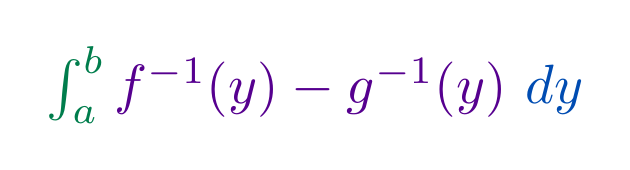
\begin{tikzpicture}[scale=2,every node/.style={transform shape}]
    \node at (0,0) {
      $\color{green!70!black!70!blue}\int_{a}^{b}\color{purple!50!blue!90!black}{f^{-1}(y) - g^{-1}(y)} \,\color{blue!70!green}{\d y}$
    };
  \end{tikzpicture}
\end{image}
could be interpreted as:
\begin{quote}
  \large\textbf{The \textcolor{green!70!black!70!blue}{sum} of the
    area of rectangles whose
    \textcolor{purple!50!blue!90!black}{widths are the difference
      between the right curve and left curve}, and whose
    \textcolor{blue!70!green}{heights are infinitesimal}.}
\end{quote}


Let's see an example.

\begin{example}
  Compute the area of the region bounded by the function $f(x) = x-3$,
  $g(x) = \sqrt{x-1}$ and the horizontal axis:
\begin{image}
\begin{tikzpicture}
	\begin{axis}[
            domain=0:5.5, ymax=2.5,xmax=5.5, ymin=0, xmin=0,
            axis lines =center, xlabel=$x$, ylabel=$y$,
            every axis y label/.style={at=(current axis.above origin),anchor=south},
            every axis x label/.style={at=(current axis.right of origin),anchor=west},
            axis on top,
          ]
          \addplot [ fill = fillp, smooth, samples=100, domain=(0:2)] ({1+x^2},{x}) \closedcycle;
          \addplot [draw=none,fill=background,domain=0:5.2] {x-3} \closedcycle;   
          \addplot [very thick, penColor2, smooth, samples=100, domain=(0:3)] ({1+x^2},{x});
          \addplot [draw=penColor,very thick,smooth] {x-3};
          
          \node at (axis cs:3.4,1.7) [penColor2] {$g$};
          \node at (axis cs:4,0.7) [penColor] {$f$};
        \end{axis}
\end{tikzpicture}
\end{image}
\begin{explanation}
  This area will be easier to compute if we look at $f^{-1}$ and $g^{-1}$. We have that
  \begin{align*}
    f^{-1}(y) &= \answer[given]{y+3}\\
    g^{-1}(y) &= \answer[given]{y^2 +1}
  \end{align*}
  We also must find where $f^{-1}$ and $g^{-1}$ intersect. Write with me
  \begin{align*}
    y+3 &= y^2 +1,\\
    \answer[given]{y^2-y-2} &= 0\\
    y &= -1 \text{ or }\answer[given]{2}.
  \end{align*}
  Note that $-1$ is not relevant for this problem.  Thus the area is
  given by
  \[
  \int_{0}^{2}(y+3) - (y^2+1)\d y = \answer[given]{\frac{10}{3}}.
  \]
  \begin{hint}
    \begin{align*}
      \int_0^2 (y+3) - (y^2+1) \d y &= \int_0^2 -y^2+y+2 \d y\\
      &=\eval{\answer{\frac{-y^3}{3} + \frac{y^2}{2}+2y}}_0^2\\
      &=\answer{\frac{10}{3}}.
    \end{align*}
  \end{hint}
\end{explanation}
\end{example}

\end{document}
